
%(BEGIN_QUESTION)
% Copyright 2011, Tony R. Kuphaldt, released under the Creative Commons Attribution License (v 1.0)
% This means you may do almost anything with this work of mine, so long as you give me proper credit

Water treatment processes use chemicals called {\it flocculants} to force suspended solids to clump together and readily fall out of suspension.  Some flocculants such as polymers have the undesirable effect of lowering the water's pH value, which not only poses problems for further use of the water but also (ironically) minimizes flocculation efficiency.  In order to counter-act this decrease in pH, powdered lime may be added to the water in addition to flocculant to raise the pH level back to a more neutral value.

One way to make this counter-acting lime addition more responsive to changes in flocculant flow is to use a {\it feedforward} control strategy to pre-emptively alter lime feed rate before the change in flocculant rate has an opportunity to affect the water's pH value.  Unfortunately, someone implemented the feedforward incorrectly, as shown in this P\&ID:

$$\includegraphics[width=15.5cm]{i00436x01.eps}$$

First, identify the mistakes you see in this P\&ID, explaining how the system {\it would} behave if it were actually built and operated like this.  Then, correct all the mistakes you see in this control strategy so that the feedforward strategy will work as it should.

\vskip 20pt \vbox{\hrule \hbox{\strut \vrule{} {\bf Suggestions for Socratic discussion} \vrule} \hrule}

\begin{itemize}
\item{} Explain why someone might be inclined to sketch the control strategy in this (incorrect) manner.  The mistakes shown here are quite common, and so there is likely a logical explanation for why they are so often made!
\item{} Identify where you think {\it dynamic compensation} might best be applied in this system, after correcting the errors in this proposed feedforward control strategy.
\end{itemize}

\underbar{file i00436}
%(END_QUESTION)





%(BEGIN_ANSWER)

In this faulty system, the flocculant {\it valve position} is being used as the feedforward signal rather than the actual flocculant {\it flow rate}.  Plus, there is one more (major) error which I will leave to you to find!
 
%(END_ANSWER)





%(BEGIN_NOTES)

Corrected feedforward system:

$$\includegraphics[width=15.5cm]{i00436x02.eps}$$

The mis-placement of the summer function block constituted a severe problem, for it would make it impossible to hold the water's pH to setpoint.  Summing the pH signal with the flocculant flow signal would result in a neither-apples-nor-oranges measurement with no real-world meaning, and this measurement would be the PV for the analytical controller trying to hold to setpoint!

%INDEX% Control, strategies: feedforward
%INDEX% Process: municipal water flocculation

%(END_NOTES)


